\documentclass{article}
\title{Efficient CP Rounding using Alternating Least Squares with QR Decomposition}
\author{Alex Zhang, Grey Ballard, and Jan Van Lent}
\date{\today}
\textwidth=16.00cm 
\textheight=26.00cm 
\topmargin=0.00cm
\oddsidemargin=0.00cm 
\evensidemargin=0.00cm 
\headheight=0cm 
\headsep=0.5cm
\textheight=610pt
\usepackage{graphicx}
\usepackage{lineno,hyperref}
\usepackage{amsmath,amssymb,amsthm,enumerate,graphicx,pifont,color,tikz,yfonts,scalerel,changepage,algorithm,algpseudocode}
\usepackage{bookmark}
\usepackage{diagbox}
\usepackage{caption,subcaption}


\usetikzlibrary{positioning}
\usetikzlibrary{cd}

\usepackage{booktabs}
\usepackage{multirow}
\usepackage{tabularx}
\usepackage{array}
\usepackage{tikz}
\usepackage{cleveref}


\graphicspath{{fig/}}

\usepackage{latexsym,array,delarray,amsthm,amssymb,epsfig}
\usepackage{amsmath}
\usepackage{listings}
\lstset{
  basicstyle=\ttfamily,
  mathescape
}

\newtheorem{property}{Property}

\newcommand{\bmat}[1]{\begin{bmatrix} #1 \end{bmatrix}}
\newcommand{\mat}[1]{\mathbf{#1}}
\newcommand{\ten}[1]{\mathcal{#1}}
% matrix/vector/tensor/element macros
\usepackage{bm}
\newcommand{\Tra}{T}										% transpose
\newcommand{\M}[2][]{\bm{#1{\mathbf{\MakeUppercase{#2}}}}} 		% matrix
\newcommand{\Me}[3][]{\bm{#1{\mathbf{\MakeUppercase{#2}}}}({#3})} 		% matrix entry
\newcommand{\Mb}[3][]{\bm{#1{\mathbf{\MakeUppercase{#2}}}}_{#3}}       	% submatrix
\newcommand{\Mbe}[4][]{\bm{#1{\mathbf{\MakeUppercase{#2}}}}_{#3}({#4})}	% submatrix entry
\newcommand{\Ms}[3][]{\bm{#1{\mathbf{\MakeUppercase{#2}}}}^{(#3)}}       	% matrix in series
\newcommand{\Mbs}[4][]{\bm{#1{\mathbf{\MakeUppercase{#2}}}}_{#3}^{(#4)}}   % submatrix in series
\newcommand{\V}[2][]{\bm{#1{\mathbf{\MakeLowercase{#2}}}}} 		% vector
\newcommand{\Vs}[3][]{\bm{#1{\mathbf{\MakeLowercase{#2}}}}^{(#3)}} 		% vector in series
\newcommand{\Ve}[3][]{\bm{#1{\mathbf{\MakeLowercase{#2}}}}({#3})}		% vector entry
\newcommand{\T}[2][]{#1{\mathbf{\cal{#2}}}} 						% tensor
\newcommand{\Te}[3][]{#1{\mathbf{\cal{#2}}}({#3})}	
\newcommand{\kr}{\odot}
\newcommand{\kron}{\otimes}
\DeclareMathOperator*{\hada}{\scalebox{1.5}{$\ast$}}
\let\ds\displaystyle

\newcommand{\GB}[1]{\textcolor{red}{\textbf{GB}: #1}}
\newcommand{\AZ}[1]{\textcolor{blue}{\textbf{AZ}: #1}}
\algnewcommand{\IfThenElse}[3]{\State \algorithmicif\ #1\ \algorithmicthen\ #2\ \algorithmicelse\ #3} % single line: \IfThenElse{<if>}{<then>}{<else>}
\algnewcommand{\IfThen}[2]{\State \algorithmicif\ #1\ \algorithmicthen\ #2} % single line: \IfThen{<if>}{<then>}

\begin{document}



\maketitle

\section{Introduction}
The CANDECOMP/PARAFAC or canonical polyadic (CP) decomposition for tensors is a popular tool for analyzing and interpreting latent patterns that may be present in multidimensional data. 
A rank-$r$ CP decomposition of a $d$-way tensor is a sum of $r$ rank-one components, each of which is a $d$-way vector outer product.
One of the most popular methods used to compute a CP decomposition is the alternating least squares (CP-ALS) algorithm, which solves a series of linear least squares problems. 
The normal equations are typically used to solve these linear least squares problems within CP-ALS because of the structure of the coefficient matrix \cite{kolda2009tensor}. 
However, this approach is sensitive to roundoff error in the case of ill-conditioned coefficient matrices. 
Minster et al. \cite{MVLB23} propose a more numerically stable approach using QR decomposition that also exploits the structure of the coefficient matrices within the linear least squares problems.
One drawback of their more stable approach is that the computational cost is exponential in the number of modes of the tensor.
This cost is often not the bottleneck when computing CP decompositions of input tensors in dense format.
However, in the context of CP-Rounding, or computing a lower-rank CP decomposition of an input already in CP format, the exponential cost becomes the overwhelming bottleneck and renders the algorithm infeasible for large problems.
In this paper, we propose a new method based on the QR decomposition that is just as numerically stable and reduces the costs from exponential to linear in the number of modes $d$.


As we describe in \cref{sec:background}, in the context of CP-ALS, the coefficient matrix of each linear least squares problem is a Khatri-Rao product of matrices, which is a column-wise Kronecker product.
The normal equations for this linear least squares problem can exploit this Khatri-Rao structure (see \cref{sec:alg:ne} for more details).
In order to efficiently compute a QR decomposition of a matrix with this structure, we perform a sequence of QR decompositions of smaller matrices.
We illustrate the key idea with an example.
Considering a Khatri-Rao product of three matrices, we exploit the following identities, where each computed QR decomposition is denoted using underbraces:

\begin{align}
\M{A} &= \underbrace{\M{A}_1}_{{\M{Q}_1\M{R}_1}} \kr \underbrace{\M{A}_2}_{{\M{Q}_2\M{R}_2}} \kr \underbrace{\M{A}_3}_{{\M{Q}_3\M{R}_3}}   \label{eq:qr} \\ 
&= (\M{Q}_1 \kron \M{Q}_2 \kron \M{Q}_3) (\underbrace{\M{R}_1 \kr \M{R}_2}_{\M[\hat]{Q}_{12} \M[\hat]{R}_{12}} \kr \M{R}_3)  \label{eq:re} \\
&= (\M{Q}_1 \kron \M{Q}_2 \kron \M{Q}_3) (\M[\hat]{Q}_{12} \kron \M{I}) (\underbrace{\M[\hat]{R}_{12} \kr \M{R}_3}_{\M[\hat]{Q}_{123} \M{R}}).  \label{eq:pw} 
\end{align}

Following \cite{MVLB23}, we start with a (compact) QR decomposition of each individual factor in \cref{eq:qr}, as the Kronecker product of the orthonormal factors can be factored out of the Khatri-Rao product as shown in \cref{eq:re}.
Note that the Khatri-Rao product of triangular matrices is not triangular, so we do not yet have a QR decomposition of $\M{A}$.
As we detail in \cref{sec:alg:expqr}, the previous approach forms the explicit Khatri-Rao product of all triangular factors and performs a large QR decomposition with cost that is exponential in the number of factors.
Instead, we propose using a pairwise approach.
In \cref{eq:re} we form an explicit Khatri-Rao product of the first two triangular factors, compute a QR decomposition, and then factor out the orthonormal factor, leaving a Khatri-Rao product with one fewer factor matrix.
In \cref{eq:qr}, we form an explicit Khatri-Rao product of the remaining two triangular factors and compute a final QR decomposition.
This achieves a QR decomposition of the matrix $\M{A}$ where the orthonormal factor is a product of implicitly represented orthonormal matrices.
We exploit the implicit structure when applying its transpose to the target matrix of the least squares problem, as the target matrix has similar structure in the context of CP-Rounding 
The cost of the pairwise approach is linear in the number of factors; full details are given in \cref{sec:alg:pwqr}.
 
\Cref{sec:result} presents experimental results to validate the complexity analysis and numerical stability properties of our proposed algorithm.
We compare our proposed algorithm with the normal equations method and with the previously proposed QR-based algorithm to show that it is as computationally efficient as the normal equations and as numerically stable as the QR-based algorithm.
We use a sine-of-sums tensor \cite{BM02} to illustrate the differences among the algorithms, as the example yields ill-conditioned least squares problems that expose the numerical instability of the normal equations and can be scaled to large numbers of modes.
Our results show a $14\times$ speedup over the previous QR-based algorithm on a single linear least squares solve for a problem with 7 Khatri-Rao factors.
We also show that our implementation of CP-ALS using QR is actually faster than the implementation of CP-ALS in the MATLAB Tensor Toolbox \cite{TensorToolbox}, which is based on the normal equations, because our implementation uses memoization to avoid recomputation of temporary quantities.
We observe up to a $4\times$ speedup over the normal equations based CP-ALS on a 9-way tensor.
For the sine-of-sums tensors, we show that the normal equations approach breaks down completely in the presence of ill-conditioning, while our method maintains small relative errors.
We summarize our conclusions in \cref{sec:conclusion} and discuss future directions based on the proposed method.

\section{Background} 
\label{sec:background}

\subsection{CP Decomposition}
Given a $d$-way tensor $\T{X} \in \mathbb{R}^{n_1\times n_2\times \dots \times n_d}$, its
CP decomposition $\T{K}$ of rank $r \in \mathbb{N}$ can be represented as 
\begin{equation}
\label{eq:CP}
\T{X}(i_1,i_2,\dots, i_d) \approx \T{K} = \sum^{r}_{j=1} \V{\lambda}(j) \mat{A_1}(i_1,j)\mat{A_2}(i_2,j) \dots \mat{A_d}(i_d,j)
\end{equation}
for all $(i_1,i_2,\dots, i_d) \in [n_1] \otimes [n_2] \otimes [n_3] \otimes \dots \otimes [n_d]$ where $\mat{A_k} \in \mathbb{R}^{n_k \times r}$ is a factor matrix for each $k \in [d]$ and $\bm{\lambda}\in\mathbb{R}^r$ is a vector of weights. 
\Cref{fig:3d-cp-decomp} gives a visualization of a CP Decomposition for a 3-way tensor.

\begin{figure}[ht!]
\centering
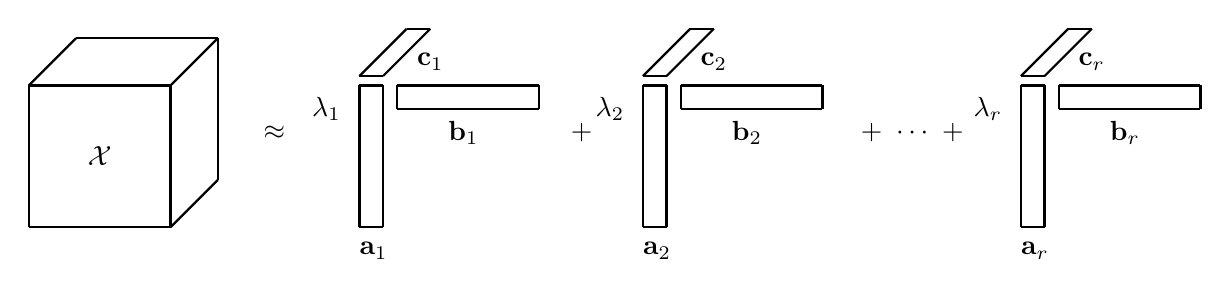
\begin{tikzpicture}[scale=0.6]
%\draw[step=1cm,gray,very thin] (0,0) grid (28,6); %grid lines

\draw node (X) at (1.5, 2.5) {$\T{X}$};
\draw[thick] (0,1) -- (3,1);
\draw[thick] (0,1) -- (0,4);
\draw[thick] (0,4) -- (3,4);
\draw[thick] (3,4) -- (3,1);
\draw[thick] (0,4) -- (1,5);
\draw[thick] (1,5) -- (4,5);
\draw[thick] (3,4) -- (4,5);
\draw[thick] (4,5) -- (4,2);
\draw[thick] (4,2) -- (3,1);

\draw node at (5.2, 3) {$\approx$};

\draw node at (6.3, 3.5) {$\lambda_1$};

\draw node at (7.3, 0.5) {$\V{a}_1$};
\draw[thick] (7,1) -- (7.5,1);
\draw[thick] (7,1) -- (7,4);
\draw[thick] (7,4) -- (7.5,4);
\draw[thick] (7.5,1) -- (7.5,4);

\draw node at (9.2, 3) {$\V{b}_1$};
\draw[thick] (7.8,3.5) -- (7.8,4);
\draw[thick] (7.8,3.5) -- (10.8,3.5);
\draw[thick] (7.8,4) -- (10.8,4);
\draw[thick] (10.8,4) -- (10.8,3.5);

\draw node at (8.5, 4.5) {$\V{c}_1$};
\draw[thick] (7,4.2) -- (7.5,4.2);
\draw[thick] (7,4.2) -- (8,5.2);
\draw[thick] (8,5.2) -- (8.5,5.2);
\draw[thick] (7.5,4.2) -- (8.5,5.2);

\draw node at (11.7, 3) {$+$};

\draw node at (12.3, 3.5) {$\lambda_2$};

\draw node at (13.3, 0.5) {$\V{a}_2$};
\draw[thick] (13,1) -- (13.5,1);
\draw[thick] (13,1) -- (13,4);
\draw[thick] (13,4) -- (13.5,4);
\draw[thick] (13.5,1) -- (13.5,4);

\draw node at (15.2, 3) {$\V{b}_2$};
\draw[thick] (13.8,3.5) -- (13.8,4);
\draw[thick] (13.8,3.5) -- (16.8,3.5);
\draw[thick] (13.8,4) -- (16.8,4);
\draw[thick] (16.8,4) -- (16.8,3.5);

\draw node at (14.5, 4.5) {$\V{c}_2$};
\draw[thick] (13,4.2) -- (13.5,4.2);
\draw[thick] (13,4.2) -- (14,5.2);
\draw[thick] (14,5.2) -- (14.5,5.2);
\draw[thick] (13.5,4.2) -- (14.5,5.2);

\draw node at (18.7, 3) {$+ \ \cdots \ +$};

\draw node at (20.3, 3.5) {$\lambda_r$};

\draw node at (21.3, 0.5) {$\V{a}_r$};
\draw[thick] (21,1) -- (21.5,1);
\draw[thick] (21,1) -- (21,4);
\draw[thick] (21,4) -- (21.5,4);
\draw[thick] (21.5,1) -- (21.5,4);

\draw node at (23.2, 3) {$\V{b}_r$};
\draw[thick] (21.8,3.5) -- (21.8,4);
\draw[thick] (21.8,3.5) -- (24.8,3.5);
\draw[thick] (21.8,4) -- (24.8,4);
\draw[thick] (24.8,4) -- (24.8,3.5);

\draw node at (22.5, 4.5) {$\V{c}_r$};
\draw[thick] (21,4.2) -- (21.5,4.2);
\draw[thick] (21,4.2) -- (22,5.2);
\draw[thick] (22,5.2) -- (22.5,5.2);
\draw[thick] (21.5,4.2) -- (22.5,5.2);
\end{tikzpicture}


\caption{CP decomposition of rank $R$ for a three-dimensional tensor $\T{X}$ \label{fig:3d-cp-decomp}}
\end{figure}
We can represent $\T[]{K}$ in shorthand CP notation as $\T{K} = [\![\V{\lambda};\mat{A}_1,\mat{A}_2, \dots,\mat{A}_d ]\!]$. 
There exists ambiguity in the weighting of the columns of the factor matrices and $\V{\lambda}$ vector.
For simplicity of presentation, we drop the weight vector $\V{\lambda}$ throughout and use the representation
$$\T{K} = [\![\mat{A}_1,\mat{A}_2, \dots,\mat{A}_d ]\!].$$

A tensor unfolding is a reshaping of the tensor elements into a matrix; mode-wise unfoldings map tensor fibers of a particular mode to columns of a matrix.
In the case of CP-format tensors like $\T{K}$, the $k$th mode-wise unfolding can be expressed in terms of the factor matrices:
$$\mat{K}_{(k)} = \mat{A}_k (\mat{A}_N \odot \dots \odot \mat{A}_{k+1} \odot \mat{A}_{k-1} \odot \dots \odot \mat{A}_1)^\top,$$
where $\odot$ denotes the Khatri-Rao product.

We use the following useful property of Khatri-Rao products:
\begin{property}
\label{prop:krnkrp}
Given matrices $\mat{A},\mat{B},\mat{C},\mat{D}$ with compatible dimensions, 
$$\mat{A}\mat{B} \odot \mat{C}\mat{D} = (\mat{A} \otimes \mat{C}) (\mat{B} \odot \mat{D}).$$
\end{property}

\subsection{Linear Least Squares Problem}
\label{sec:LS}

In mathematical form, a generic linear least squares problem is given by 
\begin{equation}
\label{eq:LS}
\min_{\mat{X}}||\mat{B} - \mat{X}\mat{A}^\top||_{F}.
\end{equation}
Note that the coefficient matrix $\mat{A}$ appears on the right of the variable matrix, which is the opposite of the standard form.
We use this form to relate to the corresponding least squares problem that arises in the context of computing a CP decomposition.

Several different techniques can be used to solve this problem.
The two we consider here are via the Normal Equations (NE) and by QR decomposition.
The NE specify a (square) linear system of equations and are derived from setting the gradient of the objective function from \cref{eq:LS} to zero, and they involve the Gram of $\mat{A}$ as well as the product $\mat{B}\mat{A}$:
\begin{equation}
\label{eq:NE}
\mat{X}\mat{A}^\top\mat{A} = \mat{B}\mat{A}.
\end{equation}
The NE can be solved via Cholesky factorization of $\mat{A}^\top\mat{A}$ and triangular solves.
The cost of NE depends on the size of $\mat{A}$ and $\mat{B}$. 

In the QR decomposition approach, we first compute the compact QR decomposition $\mat{A} = \mat{Q}\mat{R}$ (so that $\mat{Q}\in \mathbb{R}^{m \times n}$) and then solve the  triangular system
\begin{align}
\label{eq:QR}  
\mat{X} \mat{R}^\top = \mat{B}\mat{Q}.
\end{align}
For $\mat{A} \in \mathbb{R}^{m \times n}$ and $\mat{B} \in \mathbb{R}^{p \times m}$, the time complexity of each step of Normal Equations and QR decomposition is given in \cref{tab:QR-NE-time}.
Note that the cost of the QR decomposition assumes that Householder QR is used in the factorization and that the $\mat{Q}$ matrix is formed explicitly.
If $p$ is smaller than $n$, then it is more efficient to leave $\mat{Q}$ in implicit Householder form, reducing the cost of QR to $2mn^2-2/3 \,n^3$.
In this case, we apply $\mat{Q}$ to $\mat{B}$ using Householder transformations, which increases the cost of computing $\mat{B}\mat{Q}$ to $4mnp$. 


\begin{table}[!ht]
  \centering
  \begin{tabular}{|c|c|c|c|}
    \hline
    \multicolumn{2}{|c|}{\textbf{Normal Equations}} & \multicolumn{2}{c|}{\textbf{QR Decomposition}} \\
    \hline
    Component & Number of flops & Component & Number of flops\\
    \hline
    Compute Gram & $mn^2$ & Compute QR & $4mn^2 - 4/3 \, n^3$\\
    Compute $\mat{B}\mat{A}$ & $2mnp$ & Compute $\mat{B}\mat{Q}$ & $2mnp$\\
    Cholesky factorization & $1/3 \, n^3$  & N/A & \\
    Back solves & $2pn^2$  & Back solves & $pn^2$  \\
    \hline
  \end{tabular}
  \caption{Breakdown of time for using NE and QR to solve \cref{eq:LS} for $\mat{A} \in \mathbb{R}^{m \times n}$ and $\mat{B} \in \mathbb{R}^{p \times m}$}
  \label{tab:QR-NE-time}
\end{table}


If $\mat{B}$ has few columns ($p\ll n$), NE is cheaper because of the smaller coefficient in the leading order cost ($mn^2$ vs $2mn^2$). 
However, when $\mat{B}$ has many columns ($p\gg n$), the largest cost is computing $\mat{B}\mat{A}$ for NE and $\mat{B}\mat{Q}$ for QR factorization, which have leading order cost with the same constant ($2mnp$).

Using QR is more numerically stable than NE. 
Let $\kappa = \sigma_1(\mat{A})/\sigma_n(\mat{A})$ be the standard condition number of $\mat{A}$.
If we use QR to solve a least squares problem with a single right hand side; i.e. $\min\|\mat{A}\V{x} - \V{b} \|$, then from \cite[Eq. (19.2)]{trefethen1997numerical} the relative forward error satisfies
\begin{equation}\label{eq:ne-ferr}
  \frac{||\V[\tilde]{x} - \V{x}||}{||\V{x}||} = O \biggl(\biggl(\kappa + \frac{\kappa^2\tan\theta}{\eta}\biggr)\epsilon_{mach}\biggr),
\end{equation}
where $\V[\tilde]{x}$ is the computed solution, $\V{x}$ is the exact solution, $\theta$ is the angle between $\mat{A}\V{x}$ and $\V{b}$, and $\eta = \|\mat{A}\|\|\V{x}\|/\|\mat{A}\V{x}\|$.
However, if we use the NE approach, then by \cite[Eq. (19.3)]{trefethen1997numerical} the forward error guarantee can be much larger: 
\begin{equation}\label{eq:qr-ferr}
  \frac{||\V[\tilde]{x} - \V{x}||}{||\V{x}||} = O \biggl(\kappa^2 \epsilon_{\text{mach}}\biggr).
\end{equation}
Because of the numerical sensitivity introduced by using the NE approach, the QR approach is much more accurate when $\kappa$ is large (e.g., on the order of $\epsilon_{\text{mach}}^{-1/2}$ or larger) and $\theta$ is small.


\subsection{CP-ALS} \label{sec:cp-als}

\subsubsection{CP Optimization Problem}

When computing a rank-$r$ CP approximation $\T{K}$ for a $d$-way tensor $\T{X}$, we seek to minimize $\| \T{X} - \T{K} \|$, where the tensor norm generalizes the vector 2-norm or the matrix Frobenius norm.
Expressed using \cref{eq:CP}, we have  
$$\min_{\mat{A}_1,\mat{A}_2, \dots,\mat{A}_d} \| \T{X} - \T{K} \|^2 = \min_{\mat{A}_1,\mat{A}_2, \dots,\mat{A}_d} \sum_{i_1=1}^{n_1} \cdots \sum_{i_d=1}^{n_d} \left(\T{X}(i_1,i_2,\dots, i_d) - \sum^{r}_{j=1} \mat{A_1}(i_1,j)\mat{A_2}(i_2,j) \dots \mat{A_d}(i_d,j) \right)^2. $$
However, this is a nonlinear, nonconvex optimization problem and no closed form solution exists. 
We must resort to using iterative methods to approximate a solution \cite{kolda2009tensor}.

\subsubsection{CP-ALS}

One of the most effective algorithms for computing a CP decomposition of a tensor is called Alternating Least Squares (CP-ALS).
The algorithm works as a block coordinate descent method, where each block of variables is a factor matrix.
That is, it alternates over the factor matrices, holding all but one fixed and computing the optimal solution for the variable matrix.

We can solve each subproblem directly because it is a linear least squares problem.
In updating the $n$th factor matrix, we expose the linear least squares problem by unfolding $\T{X}$ and $\T{K}$ along the $k$th mode:
\begin{align}
\label{eq:cp-als-sub}
\min_{\mat{A}_k}||\T{X} - \T{K}|| &= \min_{\mat{A}_k}||\mat{X}_{(k)} - \mat{K}_{(k)}||_F \notag \\ 
&=  \min_{\mat{A}_k}||\mat{X}_{(k)} - \mat{A}_k(\mat{A}_N \odot \dots \odot \mat{A}_{k+1} \odot \mat{A}_{k-1} \odot \dots \odot \mat{A}_1)^\top||_F \notag \\ 
&=  \min_{\mat{A}_k}\|\mat{X}_{(k)}-\mat{A}_k\mat{Z}_k^\top\|_F,
\end{align}
where $\mat{Z}_k=\mat{A}_N \odot \dots \odot \mat{A}_{k+1} \odot \mat{A}_{k-1} \odot \dots \odot \mat{A}_1$.
Note that the coefficient matrix $\mat{Z}_k^\top$ appears on the right of the variable matrix, matching the generic formulation in \cref{eq:LS}.
All of the algorithms we consider in this report are based on CP-ALS, but they differ in how they solve the linear least squares subproblems specified in \cref{eq:cp-als-sub}.

\subsubsection{CP-Rounding}
\label{sec:cp-rounding}

In many applications, we wish to compute a CP decomposition of a tensor that is already in CP format, sometimes referred to as a Kruskal tensor.
That is, we wish to compute a lower-rank representation of the input tensor, sometimes referred to a CP-Rounding.
If $\T{X} \in \mathbb{R}^{n_1 \times \dots \times n_d}$ is a CP-format tensor with rank $s$, it can be written as 
$$\T{X}(i_1,i_2,\dots, i_d) = \sum^{s}_{j=1} \mat{B}_1(i_1,j)\mat{B}_2(i_2,j) \dots \mat{B}_d(i_d,j)$$
with shorthand notation $\T{X} = [\![\mat{B}^{(1)}, \dots ,\mat{B}^{(d)}]\!]$.

In the case the input tensor is in CP format, we can then utilize its special mode-$k$ unfolding representation 
$$\mat{X}_{(k)} = \mat{B}_k(\mat{B}_d \odot \dots \mat{B}_{k+1} \odot \mat{B}_{k-1} \odot \dots \odot \mat{B}_1)^\top$$
when solving the linear least squares problem given in \cref{eq:cp-als-sub}. 
That is, the least squares subproblem is given by 
\begin{equation}
\label{eq:cp-als-sub-ktensor}
\min_{\mat{A}_k}\|\mat{B}_{k}\mat{Y}_k^\top-\mat{A}_k\mat{Z}_k^\top\|_F,
\end{equation}
where $\mat{Y}_k = \mat{B}_N \odot \dots \odot \mat{B}_{k+1} \odot \mat{B}_{k-1} \odot \dots \odot \mat{B}_1$.
This structure can be exploited in different ways depending on how the least squares problem is solved.


\section{Algorithms} 
\label{sec:algo}

We now present three versions of the CP-ALS algorithm and compare their complexities.
\Cref{sec:alg:ne} presents the standard approach based on the normal equations, \cref{sec:alg:expqr} presents an existing approach that uses QR decomposition, and our proposed algorithm is detailed in \cref{sec:alg:pwqr}.
We consider general $d$-way tensors with dimensions $n_1 \times \cdots \times n_d$, and we use $r$ to denote the rank of the CP approximation.
In the case of CP-format input, we use $s$ to denote the input rank.
For complexity analysis, we use notation for arithmetic average ($\bar n$) as well as geometric mean ($\hat n$) of the tensor dimensions, which means the number of dense input tensor entries is $\hat n^d$ and the number of entries in the CP decomposition is $d\bar n r$.
Summaries of the per-iteration complexity of each algorithm are given in \cref{tab:dense_its_part} (for dense input) and \cref{tab:kruskal_its_part} (for CP format input).

\begin{table}[!ht] 
  \centering
  \begin{tabular}{|c|c|c|c|c|c|}
    \hline
    \multicolumn{2}{|c|}{\textbf{Normal Equations}} & \multicolumn{2}{c|}{\textbf{Explicit QR}} & \multicolumn{2}{c|}{\textbf{Pairwise QR}} \\
    \hline
    Component & Cost & Component & Cost & Component & Cost \\
    \hline
    Compute RHS &$2d \hat{n}^d r$ &Multi-TTM &$2d\hat n^d r$  & Multi-TTM &$2d\hat n^d r$  \\
    Compute Gram & $d^2r^2 + 3d \bar{n} r^2$&QR on factor matrices & $4d \bar n r^2$ & QR on factor matrices & $4d \bar n r^2$\\
     & &Compute $\mat{Q}_0$ & $4dr^{d+1}$& Compute pairwise $\M[\hat]{Q}$ & $4d^2r^4$\\
     & &Apply $\mat{Q}_0$& $2d\bar n r^d$& Apply pairwise $\M[\hat]{Q}$ & $2d\bar n r^d$\\
    \hline
    Leading term & $2d \hat{n}^d r$ & Leading term & $2d \hat{n}^d r$ & Leading term & $2d \hat{n}^d r$ \\
    \hline
  \end{tabular}
  \caption{Per-iteration complexity of CP-ALS algorithms for dense input}
  \label{tab:dense_its_part}
\end{table}

\begin{table}[!ht] 
  \centering
  \begin{tabular}{|c|c|c|c|c|c|}
    \hline
    \multicolumn{2}{|c|}{\textbf{Normal Equations}} & \multicolumn{2}{c|}{\textbf{Explicit QR}} & \multicolumn{2}{c|}{\textbf{Pairwise QR}} \\
    \hline
    Component & Cost & Component & Cost & Component & Cost \\
    \hline
    MTTKRP & $2d\bar n rs$ &  Multi-TTM &$2d\bar n rs$  & Multi-TTM &$2d\bar n rs$  \\
    Compute Gram & $d^2r^2+3d\bar n r^2$&QR on factor matrices & $4d \bar n r^2$ & QR on factor matrices & $4d \bar n r^2$\\
    & &Compute $\mat{Q}_0$ & $4dr^{d+1}$& Compute pairwise $\M[\hat]{Q}$ & $4d^2r^4$\\
     & &Apply $\mat{Q}_0$& $2dr^ds$& Apply pairwise $\M[\hat]{Q}$ & $2d \bar n r^ds$\\
    \hline
     Leading term & $2d\bar n rs$ & Leading term & $2dr^ds$ & Leading term & $4d\bar n rs$ \\
    \hline
  \end{tabular}
  \caption{Per-iteration complexity of CP-ALS algorithms for CP format input}
  \label{tab:kruskal_its_part}
\end{table}

\subsection{CP-ALS using Normal Equations}
\label{sec:alg:ne}

We use CP-ALS-NE to refer to the standard CP-ALS algorithm that uses the normal equations to solve the linear least squares problem given by \cref{eq:cp-als-sub} in each mode.
The normal equations for this problem are given by
\begin{equation}
  \label{eq:CP-NE}
  \mat{\hat{A}_k}\mat{Z}_k^\top\mat{Z}_k = \mat{X}_{(k)}\mat{Z}_k.
\end{equation}
The coefficient matrix $\mat{Z}_k^\top\mat{Z}_k$ can be computed as a Hadamard product of Gram matrices of the Khatri-Rao factors:
\begin{equation*}
\mat{Z}_k^\top\mat{Z}_k %= (\mat{A}_N \odot \dots \odot \mat{A}_{k+1} \odot \mat{A}_{k-1} \odot \dots \odot \mat{A}_1)^\top(\mat{A}_N \odot \dots \odot \mat{A}_{k+1} \odot \mat{A}_{k-1} \odot \dots \odot \mat{A}_1) 
= \mat{A}_d^\top \mat{A}_d \hada \cdots \hada \mat{A}_{k+1}^\top\mat{A}_{k+1} \hada \mat{A}_{k-1}^\top\mat{A}_{k-1} \hada \cdots \hada \mat{A}_{1}^\top\mat{A}_{1}.
\end{equation*}
The right hand side matrix $\mat{X}_{(k)}\mat{Z}_k$ is computed as a matricized tensor times Khatri-Rao product (MTTKRP).
Pseudocode for CP-ALS-NE is given in \cref{alg:cp-als-ne}.

\begin{algorithm}[!ht]
  \caption{CP-ALS-NE}
  \label{alg:cp-als-ne}
  %!TEX root = ../Summer-Report.tex

\begin{algorithmic}[1]\footnotesize
    
    \Function{$\{\M{A}_{k}\}=$ CP-ALS-NE}{$\T{X},r$}
      \For{$k = 1, \dots, d$}
        \State Initialize $\mat{A}_k$
        \State $\mat{G}_k = \mat{A}_k^\top\mat{A}_k$ \Comment{compute Gram}
      \EndFor
      \While{not converged}
          \For{$k = 1, \dots, d$}
              \State $\mat{H}_k = \mat{G}_d \hada \cdots \mat{G}_{k+1} \hada \mat{G}_{k-1} \cdots \hada \mat{G}_1$ \Comment{compute $\mat{Z}_k^\top \mat{Z}_k$} \label{l:NE-Hada}
              \State $\mat{M}_k = \mat{X}_{(k)}\mat{Z}_k$ \Comment{MTTKRP} \label{l:NE-mttkrp}
              \State Solve $\mat{A}_k \mat{H}_k = \mat{M}_{k}$ for $\mat{A}_k$ \Comment{via Cholesky} \label{l:NE-solve}
              \State $\mat{G}_k = \mat{A}_k^\top\mat{A}_k$ \Comment{update Gram}   \label{l:NE-Gram}
          \EndFor
      \EndWhile
    \EndFunction
    
  \end{algorithmic}
\end{algorithm}

\subsubsection{Dense Input}

When we have a dense tensor input, the dominant cost of each subiteration comes from the MTTKRP computation of $\mat{M}_k = \mat{X}_{(k)}\mat{Z}_k$ in \cref{l:NE-mttkrp}, which has leading order arithmetic cost of $2\hat n^dr$.
Computing $\mat{H}_k$ in \cref{l:NE-Hada} requires $O(dr^2)$ operations, solving the normal equations in \cref{l:NE-solve} costs $O(r^3+n_kr^2)$, and computing the Gram matrix in \cref{l:NE-Gram} costs $O(n_kr^2)$.
Thus, the sum of an entire CP-ALS-NE iteration (updating all factor matrices once) is given by
\begin{equation*}
2d\hat n^dr + O(d\bar n r^2 + d^2r^2 + dr^3).
\end{equation*}
We note that the leading order term can be reduced to $4\hat n^d r$ and the $O(d^2r^2)$ term can be reduced to $O(dr^2)$ using memoization \cite{phan2013fast}. 

\subsubsection{CP Format Input}

If the input tensor $\T{X}=[\![\mat{B}^{(1)}, \dots ,\mat{B}^{(d)}]\!]$ is already in CP format (see \cref{sec:cp-rounding}), we can compute the MTTKRP more efficiently using the following identity:
\begin{align*}
  \mat{X}_{(k)}\mat{Z}_k &= \mat{B}_k(\mat{B}_d \odot \dots \odot \mat{B}_{k+1} \odot \mat{B}_{k-1} \odot \dots \odot \mat{B}_1)^\top(\mat{A}_d \odot \cdots \mat{A}_{k+1} \odot \mat{A}_{k-1} \odot \cdots \odot \mat{A}_1) \\
 &= \mat{B}_k((\mat{B}_d^\top\mat{A}_d) \hada \cdots \hada (\mat{B}_{k+1}^\top\mat{A}_{k+1}) \hada (\mat{B}_{k-1}^\top\mat{A}_{k-1}) \hada \cdots \hada (\mat{B}_1^\top\mat{A}_1)).  
\end{align*}

\begin{algorithm}[!ht]
  \caption{CP-Round-ALS-NE}
  \label{alg:cp-als-ne-k}
  %!TEX root = ../Summer-Report.tex

\begin{algorithmic}[1]
    \Function{$\{\M{A}_{k}\}=$ CP-Round-ALS-NE}{$\{\M{B}_{k}\},r$}
      \For{$k = 1, \dots, d$}
        \State Initialize $\mat{A}_k$
        \State $\mat{G}_k = \mat{A}_k^\top\mat{A}_k$ \Comment{compute Gram}
        \State $\mat{C}_k = \mat{B}_k^\top\mat{A}_k$ \Comment{compute cross product} \label{l:round-ne-cross}
       \EndFor
    
    \While{not converged}
    \For{$k = 1, \dots, d$}
      \State $\mat{H}_k = \mat{G}_d \hada \cdots \mat{G}_{k+1} \hada \mat{G}_{k-1} \cdots \hada \mat{G}_1$ \Comment{compute $\mat{Z}_k^\top \mat{Z}_k$} 
      \State $\mat{D}_k = \mat{B}_k(\mat{C}_d \hada \cdots \mat{C}_{k+1} \hada \mat{C}_{k-1} \cdots\hada \mat{C}_1)$ \Comment{compute $\mat{X}_{(k)}\mat{Z}_n}$ \label{l:round-ne-rhs}
      \State Solve $\mat{A}_k \mat{H}_k = \mat{D}_{k}$ for $\mat{A}_k$ \Comment{via Cholesky} \label{l:NE-K-solve}
      \State $\mat{G}_k = \mat{A}_k^\top\mat{A}_k$ \Comment{update Gram}   \label{l:NE-K-Gram}
      \State $\mat{C}_k = \mat{B}_k^\top\mat{A}_k$ \Comment{update cross product}   \label{l:NE-K-cross}
    \EndFor
    \EndWhile
    \EndFunction
  \end{algorithmic} 
\end{algorithm}


When the input is a CP-format tensor of rank $s>r$, the cost is dominated by the computation of the right hand side of the normal equations.
These costs, incurred in \cref{l:round-ne-rhs,l:NE-K-cross}, are $2n_krs+(d-2)rs$ and $n_krs$ in mode $k$, respectively.
Computing the coefficient matrix of the normal equations occurs in \cref{l:round-ne-gram,l:NE-K-Gram} and has costs $(d-2)r^2$ and $n_kr^2$ in mode $k$.
Solving the normal equations in \cref{l:NE-K-solve} costs $2n_kr^2 + O(r^3)$.
Thus, the sum of an entire CP-Round-ALS-NE iteration (updating all factor matrices once) is given by
\begin{equation*}
2d\bar{n}rs + 3d\bar{n}r^2 + O(d^2rs + d^2r^2 + r^3).
\end{equation*}
We note that the $O(d^2rs+d^2r^2)$ terms can be reduced to $O(drs+dr^2)$ using memoization.
We also note that in the current implementation of this algorithm in the Tensor Toolbox \cite{TensorToolbox}, the $\mat{C}_k$ matrices are recomputed $d-1$ times per iteration. 


\subsection{CP-ALS using Explicit QR}
\label{sec:alg:expqr}

The approach proposed by Minster et al. \cite{MVLB23}, which we refer to as CP-ALS-Explicit-QR, uses the more stable QR decomposition for solving least square problem instead of the normal equations.
Consider the least squares problem in mode $k$ given by \cref{eq:cp-als-sub}.
The algorithm first performs QR on each factor matrix in $\mat{Z}_k$, which by \cref{prop:krnkrp} yields
\begin{align*}
  \mat{Z}_k &= \mat{A}_d \odot \dots \odot \mat{A}_{k+1} \odot \mat{A}_{k-1} \odot \dots \odot \mat{A}_1 \\
  &= (\mat{Q}_d\mat{R}_d) \odot \dots \odot (\mat{Q}_{k+1}\mat{R}_{k+1}) \odot (\mat{Q}_{k-1}\mat{R}_{k-1}) \odot \dots \odot (\mat{Q}_1\mat{R}_1)  \\
  &= (\mat{Q}_d \otimes \dots \otimes \mat{Q}_{k+1} \otimes \mat{Q}_{k-1} \otimes \dots \otimes \mat{Q}_1)(\mat{R}_d \odot \dots \odot \mat{R}_{k+1} \odot \mat{R}_{k-1} \odot \dots \odot \mat{R}_1).  
\end{align*}
Then it performs QR again on the Khatri-Rao product of triangular factors, obtaining $\mat{Q}_0\mat{R}_0= (\mat{R}_d \odot \dots \odot \mat{R}_{k+1} \odot \mat{R}_{k-1} \odot \dots \odot \mat{R}_1)$, so that $\mat{Z}_k = (\mat{Q}_d \otimes \dots \otimes \mat{Q}_{k+1} \otimes \mat{Q}_{k-1} \otimes \dots \otimes \mat{Q}_1)\mat{Q}_0\mat{R}_0$.
%The triangular system for QR in this case will be 
%\begin{equation}
 % \hat{\mat{A}}_k\mat{R}_0^\top = \mat{X}_{(k)}(\mat{Q}_d \otimes \dots \otimes \mat{Q}_{k+1} \otimes \mat{Q}_{k-1} \otimes \dots \otimes \mat{Q}_1)\mat{Q}_0 
%  \label{eq:CP-EXP-QR}
%\end{equation}
To solve the least square problem, we first apply the Kronecker product of orthonormal factors $\mat{Q}_d \otimes \dots \otimes \mat{Q}_{k+1} \otimes \mat{Q}_{k-1} \otimes \dots \otimes \mat{Q}_1$ to $\mat{X}_{(k)}$ from the right:
$$\mat{Y}_{(k)} = \mat{X}_{(k)}(\mat{Q}_d \otimes \dots \otimes \mat{Q}_{k+1} \otimes \mat{Q}_{k-1} \otimes \dots \otimes \mat{Q}_1),$$
which is equivalent to $\T{Y}=\T{X} \times_1 \mat{Q}_1^{\top} \cdots \times_{k-1} \mat{Q}_{k-1}^{\top}\times_{k+1} \mat{Q}_{k+1}^{\top} \cdot \times_{d} \mat{Q}_{d}^{\top}$, a Multi-TTM computation.
Then we apply the $\mat{Q}_0$ to $\mat{Y}_{(k)}$ from the right and solve the linear system via back substitution.

\begin{algorithm}
  \caption{CP-ALS-QR-Exp}
  \label{alg:cp-als-qr}
  \begin{algorithmic}[1]
    \Function{$[\bm{\lambda},\M{A}_{n}]=$ CP-ALS}{$\T{X},R$}
      \State Setup factor matrices  $\mat{A}_1$, $\mat{A}_2$, $\dots$, $\mat{A}_n$
      \State Compute QR decomposition for factor matrices $\mat{Q}_N\mat{R}_N, \dots \mat{Q}_1\mat{R}_1$
      \While{not converge}
      \For{$n = 1, \dots, N$}
      %\State Compute QR factorization $\mat{Q}_0\mat{R}_0$ for Khatri-Rao product of $\mat{R}_N, \dots, \mat{R}_1$
      \State $[\mat{Q}_0,\mat{R}_0] = \Call{QR}{\mat{R}_N \odot \cdots \odot \mat{R}_1}$
      \State $\T{Y} =  \T{X} \times_1 \mat{Q}_1^\top \dots \times_{n-1} \mat{Q}_{n-1}^\top \times_{n+1} \mat{Q}_{n+1}^\top \dots \times_N \mat{Q}_N^\top$ \Comment{Multi-TTM} \label{l:TTM}
      \State $\mat{U}_n = \mat{Y}_{(n)}\mat{Q}_0$ \label{l:apply}
      \State Solve $\mat{\hat{A}_n} = \mat{R}_0^\top \text{\textbackslash} \mat{U}_n$
      \State Update $\mat{A}_n$ and $\bm{\lambda}$
      \State Update QR for $\mat{A}_n = \mat{Q}_n\mat{R}_n$      
      \EndFor
      \EndWhile
    \EndFunction
  \end{algorithmic}
\end{algorithm}

\subsubsection{Dense Input}

Pseudocode for CP-ALS-QR for dense input is shown in \cref{alg:cp-als-qr}.
For dense input, the computation of each subiteration is dominated by \cref{l:EXP-TTM}, which is a multiple tensor-times-matrix (Multi-TTM) computation to form $\T{Y}$ with cost
$2\hat{n}^dr+O(\hat{n}^{d-1}r^2 + \cdots + \hat{n}r^d)$, where we assume the Multi-TTM is performed in order of largest mode to smallest (the largest mode is at least the geometric mean).
The cost of the QR of the Khatri-Rao product of triangular factors in \cref{l:EXP-QR-R} is $4r^{d+1}+O(r^3)$, where we assume $\mat{Q}_0$ is formed explicitly.
The cost of multiplying $\mat{Q}_0$ by $\mat{Y}_{(k)}$ in \cref{l:apply} is $2n_kr^d$.
Solving the triangular system in \cref{l:cp-als-q-exp:solve} costs $n_kr^2$, and computing the QR of the factor matrix in \cref{l:cp-als-q-exp:updateQR} is $4n_kr^2+O(r^3)$, where again we form the orthogonal factor explicitly.
%
%$$\T[]{Y} = \T[]{X} \times_1 \mat{Q}_1^\top \times \dots \times_{k-1} \mat{Q}_{k-1}^\top \times_{k+1}\mat{Q}_{k+1}^\top \times \dots \times_d \mat{Q}_d^\top$$
%and use matricized tensor $\mat{Y}_{(k)}$ times $\mat{Q}_0$.
%The computation of QR for factor matrices in \cref{l:qr_factor_q} takes $(d-2)r^2\bar{n}$. 
%The QR for Khatri-Rao product of $\mat{R}$ in \cref{l:EXP-QR-R} takes $O(r^{d+1})$ overall. 
%The cost for doing Multi-TTM will be $\hat{n}^dr$ and $\mat{U}_k = \mat{Y}_{(k)}\mat{Q}_0$ in \cref{l:apply} will be $\bar{n}r^d$.
Overall, the cost of updating factor matrices along all modes for CP-ALS-QR-Exp is
$$2d\hat{n}^dr + O(d\hat{n}^{d-1}r^2 + \cdots + d\hat{n}r^d + d\bar{n}r^d+ dr^{d+1} + d\bar{n}r^2 + dr^3 ).$$
Note that the leading order term (and several others) can be reduced by a factor of $O(d)$ using memoization \cite{KR19}.

\subsubsection{CP Format Input}
\label{sec:expqr:cpinput}

In the case of a CP format tensor input, the right hand side is computed more cheaply by applying \cref{prop:krnkrp} in reverse:
\begin{equation*}
 \mat{X}_{(k)}(\mat{Q}_d \otimes \dots \otimes \mat{Q}_{k+1} \otimes \mat{Q}_{k-1} \otimes \dots \otimes \mat{Q}_1) = 
 \mat{B}_k(\mat{Q}_d^\top\mat{B}_d \odot \cdots \odot \mat{Q}_{k+1}^\top\mat{B}_{k+1} \odot \mat{Q}_{k-1}^\top\mat{B}_{k-1} \odot \cdots \odot \mat{Q}_1^\top\mat{B}_1)^\top.
\end{equation*}
The next step of applying $\mat{Q}_0$ to the Khatri-Rao product of cross-products $\{\mat{Q}_k^\top\mat{B}_k\}$ is performed using the MTTKRP computational kernel, where we treat the dense matrix $\mat{Q}_0$ as a matricized tensor, and the final computation to compute the right hand side is a small multiplication with $\mat{B}_k$.
The algorithm is given in \cref{alg:cp-als-qr-k}.

\begin{algorithm}[!ht]
  \caption{CP-Round-ALS-QR-Exp}
  \label{alg:cp-als-qr-k}
  \begin{algorithmic}[1]
    \Function{$\{\M{A}_{n}\}=$ CP-ALS-EXPLICIT-QR-KRUSKAL}{$\T{X},r$}
      \For{$l = 1,\dots, d$}
      \State Init $\mat{A}_l$
      \State $[\mat{Q}_l,\mat{R}_l] = \Call{QR}{\mat{A}_l}$ \Comment{Factor QR}
        \State $\mat{C}_l = \mat{B}_l^\top\mat{Q}_l$ \Comment{Update $\mat{Y}_{(k)}$} \label{l:EXP-K-Apply}

      \EndFor
      \While{not converge}
      \For{$k = 1, \dots, d$}
      
      \State $\mat{U}_k = (\mat{C}_d \odot \cdots \mat{C}_{k+1} \odot \mat{C}_{n-1} \odot \cdots \mat{C}_1)\mat{Q}_0$ \Comment{MTTKRP}
      \State $\mat{U}_k = \mat{B}_k\mat{U}_k$ \Comment{matrix Mult}
      \State Solve $\mat{\hat{A}_k}\mat{R}_0^\top = \mat{U}_k$ for $\mat{A}_k$ \Comment{via TRSM}
      \State $[\mat{Q}_k,\mat{R}_k] = \Call{QR}{\mat{A}_k}$ \Comment{Update $\mat{Q}_k\mat{R}_k$}     
      \EndFor
      \EndWhile
    \EndFunction
  \end{algorithmic}
\end{algorithm}

%The cost for this algorithm is also similar to the code in dense case. However, in \cref{l:EXP-K-Apply}, the cost is $O(snr)$.
%and in \cref{l:EXP-mttkrp} the MTTKRP dominates the cost which is $(\hat{n}^dr)$.
In the case of CP format input, the costs of \cref{l:cp-round-als-exp-qr,l:cp-round-qr-solve,l:cp-round-qr-updateqr} are identical to the corresponding lines in \cref{alg:cp-als-qr}, with combined cost of $4r^{d+1}+9n_kr^2+O(r^3)$ in mode $k$.
The cost of \cref{l:EXP-mttkrp}, which we implement as an MTTKRP, is $2r^ds$.
The cost of the matrix multiplications in \cref{l:exp-finish-rhs,l:EXP-K-update-cross} together is $4n_krs$.
Thus, the overall cost of CP-Round-ALS-QR-Exp is
$$ 2dr^ds + 4dr^{d+1} + O(d\bar{n}rs+d\bar{n}r^2 + r^3).$$
Again, it is possible to reduce the leading order costs by a factor of $O(d)$ via memoization.

\subsection{CP-ALS using Pairwise QR}
\label{sec:alg:pwqr}


We now describe our proposed CP-ALS algorithm that uses the QR decomposition but avoids the explicit computation of the Khatri-Rao product of all $d-1$ triangular matrices.
That is, it avoids computing $\mat{Q}_0\mat{R}_0$ as described in \cref{sec:alg:expqr}, which has a cost that is exponential in $d$.

The first phase of the algorithm is the same: we perform QR decompositions on individual factor matrices and exploit \cref{prop:krnkrp}:
$$\mat{Z}_k = (\mat{Q}_d \otimes \dots \otimes \mat{Q}_{k+1} \otimes \mat{Q}_{k-1} \otimes \dots \otimes \mat{Q}_1)(\mat{R}_d \odot \dots \odot \mat{R}_{k+1} \odot \mat{R}_{k-1} \odot \dots \odot \mat{R}_1).$$
To compute the QR decomposition of the Khatri-Rao product of triangular factors, we perform a sequence of pairwise reductions.
While the order is arbitrary, for notational convenience we start from the right: we compute a QR decomposition of an explicit Khatri-Rao product of the last two triangular factors, $\mat{R}_2 \odot \mat{R}_1 = \M[\hat]{Q}_1\M[\hat]{R}_2$, yielding
$$\M{R}_{d-1} \odot \dots \odot \mat{R}_{k+1} \odot \mat{R}_{k-1} \odot \dots \odot \M[\hat]{Q}_1\M[\hat]{R}_2 = (\M{I}_{r^{d-2}} \kron \M[\hat]{Q}_1)(\M{R}_{d-1} \odot \cdots \odot \mat{R}_{k+1} \odot \mat{R}_{k-1} \odot \dots \odot \M[\hat]{R}_2).$$
We then repeat the pairwise QR decomposition on two rightmost remaining factors $\M{R}_{3} \odot \M[\hat]{R}_2$, and so on (skipping the $k$th factor), each time reducing the number of triangular factors by one.
After $d-2$ pairwise QR decompositions, we obtain the QR decomposition of $\mat{Z}_k$ (with implicit orthogonal factor):
$$\mat{Z}_k = (\mat{Q}_d \otimes \dots \otimes \mat{Q}_{k+1} \otimes \mat{Q}_{k-1} \otimes \dots \otimes \mat{Q}_1) (\M{I}_{r^{d-2}} \kron \M[\hat]{Q}_1)(\M{I}_{r^{d-3}} \kron \M[\hat]{Q}_2) \cdots (\mat{I}_r \otimes \M[\hat]{Q}_{d-2}) \M[\hat]{Q}_{d-1}\M{R}.$$

As in the previous approach, applying the orthogonal factor to the unfolding of the tensor $\M{X}_{(k)}$ starts with a Multi-TTM operation:
$$\T{Y} =  \T{X} \times_1 \mat{Q}_1^\top \dots \times_{k-1} \mat{Q}_{k-1}^\top \times_{k+1} \mat{Q}_{k+1}^\top \dots \times_d \mat{Q}_d^\top.$$
Applying the orthogonal factors computed during the pairwise phase differs depending on the structure of the input.

\subsubsection{Dense Input}

In the case the input $\T{X}$ is dense, $\T{Y}$ is a dense tensor with dimensions $r\times \cdots \times r \times n_k \times r \times \cdots \times r$.
Each $\M[\hat]{Q}_\ell$ (for $1\leq \ell < d$ and $\ell \neq k$) has dimension $r^2 \times r$, and postmultiplying $\M{Y}_{(k)}$ by the Kronecker product of an orthogonal factor and the identity corresponds to a contraction with two of the modes of the tensor $\M{Y}$.
To simplify the presentation of the approach in \cref{alg:cp-als-pairwise-qr}, we first permute the tensor so that the $k$th mode is last, which allows the contraction to be performed on the first two modes each time.
 
\begin{algorithm}
  \caption{CP-ALS-QR-Imp}
  \label{alg:cp-als-pairwise-qr}
  \begin{algorithmic}[1]
    \Function{$[\bm{\lambda},\M{A}_{n}]=$ CP-ALS}{$\T{X},R$}
      \State Setup factor matirces  $\mat{A}_1$, $\mat{A}_2$, $\dots$, $\mat{A}_n$
      \State Compute QR decomposition for factor matrices $\mat{Q}_N\mat{R}_N, \dots \mat{Q}_1\mat{R}_1$
      \While{not converge}
      \For{$n = 1, \dots, N$}
      \State Compute pairwise QR factorization $(\mat{Q}_{A_{N-1}} \otimes \dots  \otimes  \mat{I}_N) \dots \mat{Q}_{A_{1}}\mat{R}_{A_{1}}$ for each $\mat{R}_N, \dots, \mat{R}_1$
      \State TTM with Kruskal format $\mat{Y}_{(n)} = \mat{B}_1\mat{Q}^\top_1 \odot \dots \odot \mat{B}_{n-1}\mat{Q}^\top_{n-1}\odot \mat{B}_{n+1}\mat{Q}^\top_{n+1} \odot \dots \odot \mat{B}_N\mat{Q}^\top_N$
      \State Apply pairwise QR on $\mat{Y}_n\mat{Q}_{A_{N-1}}^\top  = (\mat{Q}_{A_{N-1}}^\top(\mat{Q}_N\mat{B}_N \odot \mat{Q}_{N-1}\mat{B}_{N-1}) \odot \dots \odot  \odot \mat{Q}_{1}\mat{B}_{1})^\top\mat{B}_n $
      
      \State Solve $  \mat{\hat{A}}_n = \mat{R}^\top_{A_1} \text{\textbackslash} \mat{B}^\top_M\mat{Q}_M\mat{B}_n $
      \State Update $\mat{A}_n$ and $\bm{\lambda}$
      \State Update QR for $\mat{A}_n = \mat{Q}_n\mat{R}_n$      
      \EndFor
      \EndWhile
    \EndFunction
  \end{algorithmic}
\end{algorithm}

The cost of the Multi-TTM in \cref{l:pairwise-TTM} is the same as in \cref{alg:cp-als-qr}: $2\hat{n}^dr+O(\hat{n}^{d-1}r^2 + \cdots + \hat{n}r^d)$.
The permutation in \cref{l:pairwise-permute} has no arithmetic cost, though in practice it may take significant time due to the high relative cost of memory movement.
The pairwise QR decompositions (\cref{l:pairwise-QR}) together cost $4(d-2)r^4 + O(dr^3)$ for mode $k$, and applying the pairwise orthogonal factors via TTM (\cref{l:pair-R-TTM}) costs a total of $2n_kr^d+2n_kr^{d-1}+\cdots+2n_kr^3$.
The triangular solve in \cref{l:pairwise-solve} costs $n_kr^2$.
The cost of the QR decomposition in \cref{l:pairwise-factorQR} is $4n_kr^2+O(r^3)$ in mode $k$.
Thus, the total cost of a full iteration (updating each factor matrix once) of CP-ALS-QR-Imp is
$$ 2d\hat{n}^d + 2d\bar{n}r^d + 4d^2r^4 + O(d\hat{n}^{d-1}r^2 + d\bar{n}r^{d-1}). $$
The leading order cost can be reduced by a factor of $O(d)$ via memoization \cite{KR19}.

\subsubsection{CP Format Input} 
\label{sec:QR-PW-k}

With CP format input, we can use the Khatri-Rao structure $\mat{X}_{(k)} = \mat{B}_{k}(\mat{B}_{d} \odot \dots \odot \mat{B}_{k+1} \odot \mat{B}_{k-1}  \odot \dots \odot \mat{B}_{1})^\top$ when applying the orthogonal factor into $\mat{X}_k$. 
As described in \cref{sec:expqr:cpinput}, this gives us
\begin{align*}
  %\mat{Y}_k &= (\mat{B}_{k}(\mat{B}_{d} \odot \dots \odot \mat{B}_{k+1} \odot \mat{B}_{k-1}  \odot \dots \odot \mat{B}_{1})^\top)(\mat{Q}_d \otimes \dots \otimes \mat{Q}_{k+1} \otimes \mat{Q}_{k-1} \otimes \dots \otimes \mat{Q}_1) \nonumber \\
  \mat{Y}_k &= \mat{B}_k(\mat{Q}_d^\top\mat{B}_d \odot \cdots \odot \mat{Q}_{k+1}^\top\mat{B}_{k+1} \odot \mat{Q}_{k-1}^\top\mat{B}_{k-1} \odot \cdots \odot \mat{Q}_1^\top\mat{B}_1)^\top \\
  &= \mat{B}_k(\mat{C}_d \odot \cdots \odot \mat{C}_{k+1} \odot \M{C}_{k-1} \odot \cdots \odot \M{C}_1)^\top.
\end{align*}
For the pairwise updates, we continue to exploit the Khatri-Rao structure.
To apply the first pairwise orthogonal factor, we use the identity
\begin{align*}
(\M{C}_d \odot \cdots \odot \M{C}_{k+1} \odot \M{C}_{k-1} \odot \cdots \odot \M{C}_3 \odot \M{C}_2 \odot \M{C}_1)^\top(\M{I}_{r^{d-2}} \otimes \M[\hat]{Q}_1) = \\
(\M{C}_d \odot \cdots \odot \M{C}_{k+1} \odot \M{C}_{k-1} \odot \cdots \odot \M{C}_3 \odot \M[\hat]{Q}_1^\top(\M{C}_2 \odot \M{C}_1))^\top = \\
\M{C}_d \odot \cdots \odot \M{C}_{k+1} \odot \M{C}_{k-1} \odot \cdots \odot \M{C}_3 \odot \M[\hat]{C}_2.
\end{align*}
That is, we form the explicit Khatri-Rao product of the last two factors (forming a dense matrix with dimensions $r^2 \times s$) and apply the pairwise orthogonal factor using matrix multiplication, which reduces the number of $r \times s$ Khatri-Rao factors by one.
In the next step, we apply the next $r^2 \times r$ pairwise orthogonal factor to the last two remaining factors, and so on.
After $d-2$ steps, we obtain a final $r\times s$ factor that is multiplied into $\M{B}_k$ to form the right hand side of the triangular linear system.
The pseudocode for this approach, where we apply the pairwise orthogonal factors as soon as we compute them, is given in \cref{alg:cp-als-pairwise-qr-kruskal}.


\begin{algorithm}
  \caption{CP-Round-ALS-QR-Imp}
  \label{alg:cp-als-pairwise-qr-kruskal}
  %!TEX root = ../Summer-Report.tex

\begin{algorithmic}[1]
    \Function{$\{\M{A}_{k}\}=$ CP-Round-ALS-QR-Imp}{$\{\M{B}_{k}\},r$}
      \For{$k = 1, \dots, d$}
        \State Initialize $\mat{A}_k$
        \State $[\mat{Q}_k,\mat{R}_k] = \Call{QR}{\mat{A}_k}$ \Comment{compute QR} 
        \State $\mat{C}_k = \mat{Q}_k^\top\mat{B}_k$ \label{l:Pair-K-Apply} \Comment{compute cross product}  
      \EndFor
      \While{not converge}
        \For{$k = 1, \dots, d$}
          \IfThenElse{$k \neq 1$}{$a=1$}{$a=2$} \Comment{set starting index}
          \State $\mat{R}_0 = \mat{R}_a$, $\mat{D}_k = \mat{C}_a$ \Comment{initialize pairwise results}
          \For{$\ell = 1, \dots, d$} 
            \If{$\ell\neq k \textbf{ and }\ell\neq a$}
              \State $[\mat{Q}_0,\mat{R}_0] = \Call{QR}{\mat{R}_\ell \odot \mat{R}_0}$ \label{l:pair-QR-R} \Comment{pairwise QR}
              \State $\mat{D}_k = (\mat{C}_\ell \odot \mat{D}_k)^\top\mat{Q}_0$ \Comment{pairwise apply}
            \EndIf
          \EndFor
          \State $\mat{U}_k = \mat{B}_k\mat{D}_k$ \Comment{via matrix multiplication}
          \State Solve $  \mat{A}_k\mat{R}_0^\top = \mat{U}_k$ for $\mat{A}_k$ \Comment{via triangular solve}    
          \State $[\mat{Q}_k,\mat{R}_k] = \Call{QR}{\mat{A}_k}$ \Comment{update QR}   
          \State $\mat{C}_k = \mat{Q}_k^\top\mat{B}_k$ \label{l:Pair-K-update} \Comment{update cross product}  
        \EndFor
      \EndWhile
    \EndFunction
  \end{algorithmic}
\end{algorithm}


For CP format input of rank $s$, we first consider the costs of the factor matrix QR decompositions and applying the individual orthogonal factors.
In mode $k$, the cost of the QR in \cref{l:Pair-K-update} is $4n_kr^2$, and the cost of applying the explicit orthogonal factor to the corresponding input factor matrix in \cref{l:Pair-K-apply} is $2n_krs$.
Performing the pairwise QR decompositions and applying the explicit orthogonal factors occurs in \cref{l:pair-QR-R,l:pair-QR-Rapply}.
For each subiteration, the cost of the two operations, which are both performed $d-2$ times, is $4dr^4+2dr^3s+O(r^4)$.
The final multiplication and triangular solve in \cref{l:Pair-K-matmul,l:Pair-K-solve} together cost $2n_krs+n_kr^2$.
Performing a full iteration and updating each factor matrix once has total cost
$$ 4d\bar{n}rs + 5d\bar{n}r^2 + 2d^2r^3s + 4d^2r^4 + O(r^4). $$
The terms involving factors of $d^2$ can likely be reduced by a factor of $d$ via memoization, but we do not consider that optimization here.

\section{Experimental Results} 
\label{sec:result}


\subsection{Sine of Sums Tensor}

To test the accuracy and efficiency of the QR-based method, we use a discretization of sine of sums: $\sin(x_1+\dots+ x_d)$.
Repeated using the textbook sine of sums and cosine of sums identities for two variables, we obtain a $2^{d-1}$-term separated representation of the function.
For example, 
\begin{equation*}
\begin{split}
\sin(x_1+x_2+x_3) = \sin(x_1)\cos(x_2)\cos(x_3)+\cos(x_1)\cos(x_2)\sin(x_3) \\
+\cos(x_1)\sin(x_2)\cos(x_3) - \sin(x_1)\sin(x_2)\sin(x_3).
\end{split}
\end{equation*}
As described in previous work \cite{BM02,MVLB23}, there exists a $d$-term separated representation of the form
\begin{equation}
\label{eq:dtermrep}
\sin\left(\sum^d_{j=1}x_j\right) = \sum^d_{j=1}\sin(x_j)\prod^d_{k=1,k\neq j}\frac{\sin(x_k - \alpha_k -\alpha_j)}{\sin(\alpha_k - \alpha_j)}
\end{equation}
for all choices of  ${\alpha_j}$ such that $\sin(\alpha_k - \alpha_j) \neq 0$ for all $j \neq k$.
Our goal is to compute this much more efficient $d$-term representation using the $2^{d-1}$-term representation numerically using discretized representations of the functions.
This corresponds to running CP-ALS with CP format input.

\subsection{Algorithm Comparison for Single Least Squares Problem}

We first compare the three methods for solving a single least squares problem where the coefficient matrix is a Khatri-Rao product and the right hand side has matching Khatri-Rao structure, as given in \cref{eq:cp-als-sub-ktensor}:
\begin{align*}
\min_{\mat{A}_k} & \; \|\mat{B}_{k}\mat{Y}_k^\top-\mat{A}_k\mat{Z}_k^\top\|_F, \text{ where} \\
\mat{Y}_k &= \mat{B}_N \odot \dots \odot \mat{B}_{k+1} \odot \mat{B}_{k-1} \odot \dots \odot \mat{B}_1 \text{ and} \\
\mat{Z}_k &= \mat{A}_N \odot \dots \odot \mat{A}_{k+1} \odot \mat{A}_{k-1} \odot \dots \odot \mat{A}_1.
\end{align*}
Here we set the right hand side factors to be discretizations of the $2^{d-1}$-term representation, using an $n$-point discretization of $[0,2\pi)$.
This implies that each $\M{B}_j$ has dimension $n \times 2^{d-1}$.
We set the coefficient matrix $\M{Z}_k$ to be a Khatri-Rao product of matrices corresponding to $n$-point discretizations of the $d$-term representation so that each $\M{A}_j$ has dimension $n\times d$. 
We choose $\alpha_j$'s to be equally spaced within $[0,2\pi)$.
Leaving one factor matrix $\M{A}_k$ out of the representation, our goal is to recompute it by solving the least squares problem.

\Cref{tab:LS_err} reports the accuracy of the three methods as we vary the condition number as measured by the relative forward error $\|\M{A}_k-\M[\hat]{A}_k\|/\|\M{A}_k\|$, where $\M{A}_k$ is the true solution given by the discretization of \cref{eq:dtermrep} and $\M[\hat]{A}_k$ is the computed solution.
We adjust the condition number of the coefficient matrix by varying $d$ and the distance between consecutive parameters $\alpha_j$ and $\alpha_j+1$, and we fix the discretization parameter $n=50$.
We observe that as the distance between consecutive parameters decreases, the condition number of the coefficient matrix increases, and this effect is more pronounced for $d=5$ than $d=3$.
As the condition number increases, we see that the forward error of all methods increases, as expected.
However, this loss of accuracy is much worse for the normal equations method, and when the condition number is a large as the reciprocal of the square root of machine precision, it completely breaks down.
For the QR-based methods, the loss of accuracy is much more graceful, and both methods maintain forward error at or below the square root of machine precision even when the condition number is on the order of \texttt{1e13}.
This experiment confirms the difference in theoretical guarantees presented in \cref{eq:ne-ferr,eq:qr-ferr}.
We note that the implicit Pairwise QR method yields slightly more accurate results than the explicit QR method, which we conjecture is due to the computations involving explicit vectors of dimension $n^{d-1}$, which the implicit method avoids.

\begin{table}[ht!] 
  \centering
  \begin{tabular}{|c|c|c|c|c|c|}
    \hline
    $d$  & $|\alpha_j-\alpha_{j+1}|$ & $\kappa(\M{Z}_k)$ & NE Err & QR Exp Err & QR Imp Err \\
    \hline
    3  & \texttt{1e00}  & \texttt{1.51e00}  & \texttt{3.64e-16} & \texttt{1.44e-15} & \texttt{5.07e-16} \\
    3  & \texttt{1e-1} & \texttt{5.02e02}  & \texttt{6.12e-14} & \texttt{3.70e-15} & \texttt{5.74e-16} \\
    5  & \texttt{1e-1} & \texttt{7.38e03}  & \texttt{9.80e-11} & \texttt{9.70e-15} & \texttt{1.85e-15}\\
    3  & \texttt{1e-2} & \texttt{4.77e05}  & \texttt{1.32e-08} & \texttt{5.40e-13} & \texttt{8.99e-15} \\
    5  & \texttt{1e-2} & \texttt{3.71e08}  & \texttt{3.51e-01} & \texttt{4.87e-12} & \texttt{1.27e-14}\\
    3  & \texttt{1e-4} & \texttt{4.77e11} & \texttt{8.89e-01} & \texttt{8.43e-09} & \texttt{1.31e-12} \\
    5  & \texttt{1e-3} & \texttt{3.64e13} & \texttt{1.00e00}  & \texttt{9.74e-07} & \texttt{1.94e-09}\\
    \hline
  \end{tabular}
  \caption{Comparison of relative forward error when varying $d$ and $|\alpha_j-\alpha_{j+1}|$ for single least squares problem given by sine of sums}
  \label{tab:LS_err}
\end{table}

\Cref{fig:LS_problem_line} reports the total time for solving the single least squares problem varying the number of modes $d$ and fixing the discretization parameter $n=2000$.
Here we observe the exponential dependence on $d$ of the explicit QR method's complexity: as $d$ increases, the time required to solve the least square problem increases drastically.
The normal equations method and the implicit QR method, with complexities that are linear in $d$, have running times that increase much more slowly with $d$ and are comparable to each other.

\begin{figure}[ht!]
  \begin{center}
    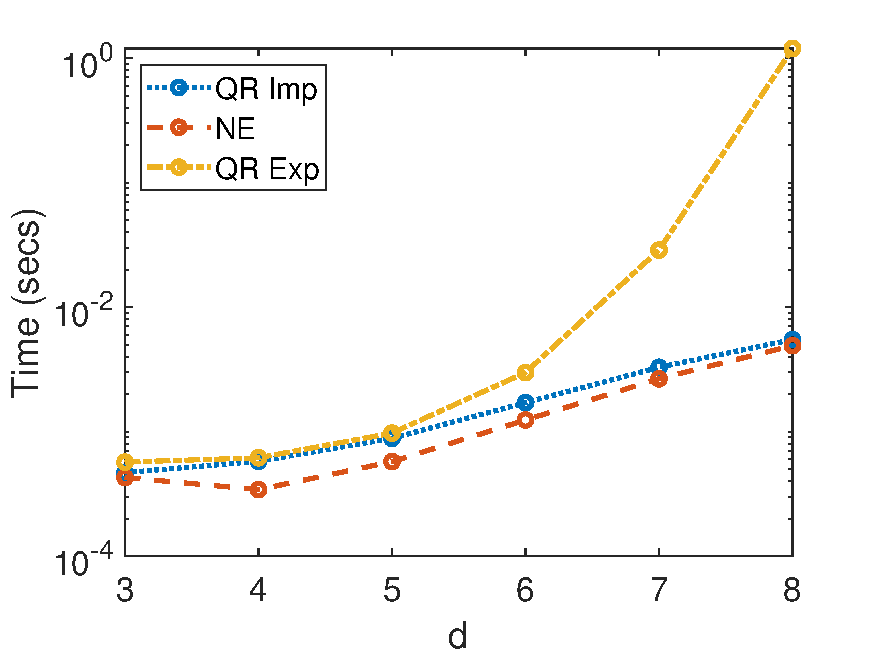
\includegraphics[scale = 0.7]{lineplot_p.pdf}
    \caption[Figure]{Comparison of run time when varying $d$ for NE, QR Imp, and QR Exp ($n=2000$) \GB{Please change the y-axis label to ``Time (secs)" and the x-axis label to ``d" and remove the title} \label{fig:LS_problem_line}}
  \end{center}
\end{figure}

In \cref{fig:LS_problem_breakdown}, we see a breakdown of the running times for the normal equations and implicit QR methods as reported in \cref{fig:LS_problem_line}.
Our first observation is that the time spent in applying the factor-wise orthonormal matrices to the right hand side and computing the right hand side of the normal equations, labeled $Q^TB/A^TB$, dominates the running time and is nearly identical between algorithms.
This confirms the argument made in \cref{sec:LS} for unstructured least squares problems with many right hand sides.
The second observation is that the time spent in factor-wise QR's is greater than that of computing Gram matrices, as they require twice the flops and are slightly less efficient.
The pairwise QR and the application of the pairwise orthonormal factors is a unique cost to the implicit QR method, and that time is the main reason that the implicit QR method is slightly slower than the normal equations method.
We also note that the linear system solve is noticeably slower for the normal equations method; we conjecture this is because Matlab is resorting to an SVD to solve a linear system it has detected is ill conditioned.

\begin{figure}[ht!]
  \begin{center}
    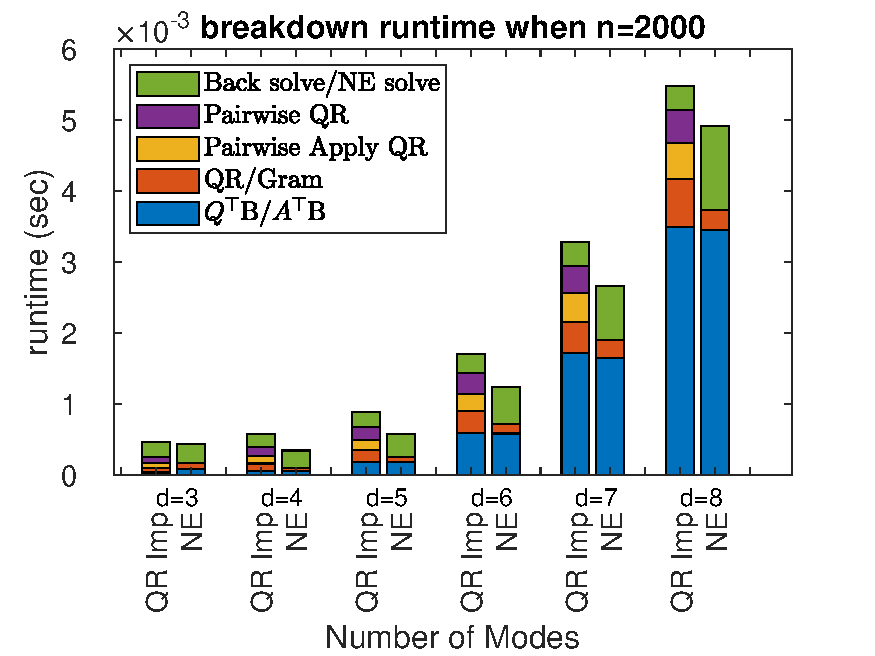
\includegraphics[scale = 0.8]{breakdown_p.pdf}
    \caption[Figure]{Breakdown of run time when varying $d$ for NE and QR Imp ($n=2000$) \GB{Please change the y-axis label to ``Time (secs)" and the x-axis label to ``d" and remove the title}\label{fig:LS_problem_breakdown}}
  \end{center}
\end{figure}

\subsection{CP-ALS Algorithm Comparisons}

In the next set of experiments, we incorporate the implicit Pairwise QR method into CP-ALS and further compare the runtime and accuracy with CP-Round-ALS-NE and CP-Round-ALS-QR-Exp. 
We use a discretized version of the $2^{d-1}$-term representation of the sine of sums tensor as input, and we initialize CP-ALS randomly.

\Cref{fig:runtime} reports the per-iteration run time of each of the three methods, varying $d\in\{3,5,7,9\}$ and $n \in \{10000,15000,30000\}$.
For 3-way tensors, the running times are comparable, though the normal equations is typically the fastest.
For larger $d$, we see that the explicit QR method's running time increases drastically due to the exponential dependence on $d$, and we did not attempt to complete the experiment for $d=9$.
While the normal equations and implicit QR methods have comparable time for $d=5$, we see the that implicit QR method outperforms NE for $d=7$ and $d=9$.
This improvement is because we use the Tensor Toolbox's implementation of CP-ALS, which performs redundant computation in the MTTKRPs.
We avoid this in our implementation of the QR-based methods, using memoization.
We note that it is possible to apply memoization to the normal equations based method, and we would expect to see comparable performance to the implicit QR method with that optimization.

\begin{figure}[ht!]
  \begin{center}
    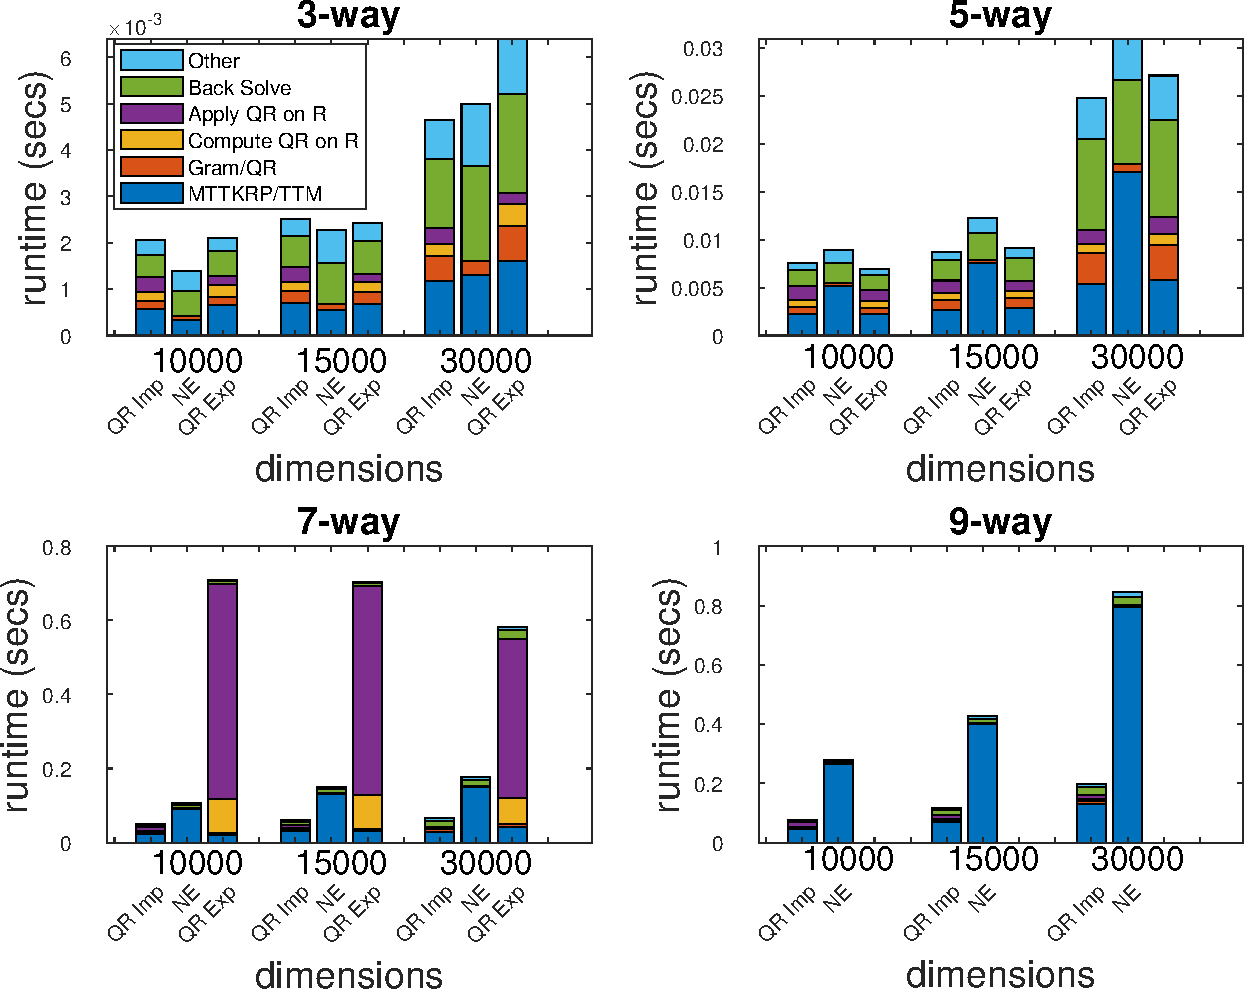
\includegraphics[scale = 0.7]{Fig_kt.pdf}
    \caption[Figure]{Comparison of per-iteration run time when varying $d$ and $n$ for NE, QR Imp and QR Exp \GB{Please change the y-axis label to ``Time (secs)" and the x-axis label to n} \label{fig:runtime}}
  \end{center}
\end{figure}


To compare the accuracy of the NE-based and implicit Pairwise QR-based CP-ALS algorithms, we perform experiments with the sine of sums input with varying numbers of modes $d\in \{5,7,10\}$ and fixed $n=10$.
\Cref{fig:error} shows the convergence behavior as measured by the relative backward/residual error over 40 iterations for two different random initializations.
We observe that overall, the QR-based method is able to achieve lower error in each of the 6 experiments.
In the case of $d=5$ and $d=7$, we observed little variability over initialization: the QR-based method converged to errors that were orders of magnitude smaller than the NE-based method, and that difference grows with $d$.
In the case of $d=10$, we observed differing behavior for different initializations, confirming previously reported observations \cite{MVLB23}: the NE-based method failed about 80\% of the time (as shown in the 2nd trial) and achieved moderately large error about 20\% of the time (as shown in the 1st trial).
The QR-based method, on the other hand, consistently converged to solutions with small residual error, illustrating its better numerical stability properties.

\begin{figure}[ht!]
  \begin{center}  
    \includegraphics*[scale = 1.1]{sinsums_acc2.pdf}
    \caption[Figure]{Comparison of convergence behavior of NE and QR Imp for varying $d$ and random initializations ($n=10$) \GB{Please change the y-axis label to ``Relative residual error"} \label{fig:error}}
  \end{center}  
\end{figure}

\section{Conclusion}
\label{sec:conclusion}

In this work, we implement a new version of CP-ALS algorithm with QR decomposition that in the case of CP-format input reduces the exponential time complexity of a previously proposed solution \cite{MVLB23} to polynomial time without sacrificing numerical stability.
The time complexity roughly matches that of the standard normal equations based CP-ALS algorithm as implemented in the Tensor Toolbox \cite{TensorToolbox}.
As evidenced by our theoretical and experimental analysis, the algorithm simultaneously achieves numerical stability and computational efficiency.

Our experiments with a single least squares problem show that for an ill-conditioned problem (condition number of \texttt{4e13}), our algorithm achieves an error that is 9 orders of magnitude smaller than the normal equations approach.
Likewise, for an 8-way tensor, we observe a speedup of about $100\times$ over the previously proposed QR-based method.
In experiments using CP-ALS to perform CP rounding, we observe a $14\times$ speedup over the previous QR-based method on a 7-way tensor and $4\times$ speedup over Tensor Toolbox's implementation of the NE-based method.
Further, we also see convergence to more accurate solutions when using our method for $5$-way, $7$-way, and $10$-way tensors correspond to discovery of a sine of sums identity.

Our future work includes implementing this QR-based method within Tensor Toolbox, providing a more accurate CP-ALS approach for CP-format input that does not sacrifice computational efficiency.
We also note that there are more opportunities to exploit memoization in our pairwise QR algorithm.
Finally, we believe that the pairwise QR approach can improve the cost and accuracy for computing leverage scores for randomized methods as described in \cite{bharadwaj2023fast}, which we would like to explore further.


\bibliographystyle{plain}
\bibliography{reference}

\end{document}